\documentclass[conference]{IEEEtran}
\usepackage{amsmath}
\usepackage{eurosym}
\usepackage{subcaption}
\usepackage[noadjust]{cite}
 \usepackage{graphicx}
\usepackage{algorithm, algorithmic}
\usepackage{xcolor}
\usepackage{hyperref}
\usepackage{url}
\usepackage{listings}
\lstset{basicstyle=\ttfamily,
  showstringspaces=false,
  commentstyle=\color{red},
  keywordstyle=\color{blue}
}

\usepackage{mathtools}
\usepackage{longtable}
\usepackage{array}
\usepackage{multirow}
\newcolumntype{L}[1]{>{\raggedright\let\newline\\\arraybackslash\hspace{0pt}}m{#1}}
\newcolumntype{C}[1]{>{\centering\let\newline\\\arraybackslash\hspace{0pt}}m{#1}}
\newcolumntype{R}[1]{>{\raggedleft\let\newline\\\arraybackslash\hspace{0pt}}m{#1}}
\interdisplaylinepenalty=2500


\interdisplaylinepenalty=2500
\newcommand\Mark[1]{\textsuperscript{#1}}
\newcommand\fixit[1]{{\color{red}{\Large FIX:} #1}}

\newcommand{\argmax}[1]{\underset{#1}{\operatorname{arg\,max\,}}}

\begin{document}
%
% paper title
% Titles are generally capitalized except for words such as a, an, and, as,
% at, but, by, for, in, nor, of, on, or, the, to and up, which are usually
% not capitalized unless they are the first or last word of the title.
% Linebreaks \\ can be used within to get better formatting as desired.
% Do not put math or special symbols in the title.

\title{Implementation of ZNCC algorithm for disparity map computation using OpenCL}

\author{
    \IEEEauthorblockA{{\normalfont\large Aleksei~Tiulpin}\\Center for Machine Vision and Signal Analysis\\University of Oulu}
    \and
    \IEEEauthorblockA{{\normalfont\large Iaroslav~Melekhov}\\Department of Computer Science\\ Aalto University}
}


\maketitle


\begin{abstract}
In this report we describe an implementation of zero mean cross-correlation algorithm for stereo correspondence search. In particular, we show the accelerated implementation of the algorithm using OpenCL v.1.2 standard. The performance gain which we managed to achieve with the accelerated version of the algorithm is around 100 times.
\end{abstract}


\section{Introduction}
Estimation of a disparity map of an image sequence plays important role in such large areas of computer vision as multi-view image generation, 3D reconstruction from stereo image pairs and object recognition~\cite{Redert99, arsenio97}. Obtaining a precise and accurate depth map is the ultimate goal in these applications.

By the definition, binoclular disparity is positional difference between the two retinal projections of a given point in space. This positional difference is a result of the fact that the two eyes are laterally separated and therefore see the world from two slightly different vantage points \cite{Qian1997359}.

Many different approaches have been developed to estimate the disparity field \cite{Redert99}, however in this work we focus on one of the area-based algorithm for the disparity map estimation -- zero mean cross correlation (ZNCC)~\cite{aschwanden92}. In addition, we will show how to apply several post-processing techniques in order to compute the depth map out of two disparity fields. 

The benefit of the ZNCC algorithm is a simple and straightforward implementation, which is moreover well suited for data-parallel acceleration using Graphical Processing Units (GPU). In our work, OpenCL standard v.1.2 has been used for this purpose. In addition, we have performed a series of experiments and optimized our implementation for NVIDIA GPU.

The report is organized as follows. In Section~\ref{sec:CbasedImplementation} ZNCC algorithms implemented in C language is presented. Section~\ref{sec:OpenclImplementation} describes the proposed method of calculating disparity map based on OpenCL technology. Section~\ref{sec:Benchmarks} presents benchmarks of the algorithm evaluated on two different GPU. In Section~\ref{sec:Optimization} we briefly discuss about OpenCL optimization and a way how to improve performance further. In the end of this report we summarize our results.

\begin{figure}[t!]
\centering
	\begin{subfigure}{0.49\linewidth}
		\centering
		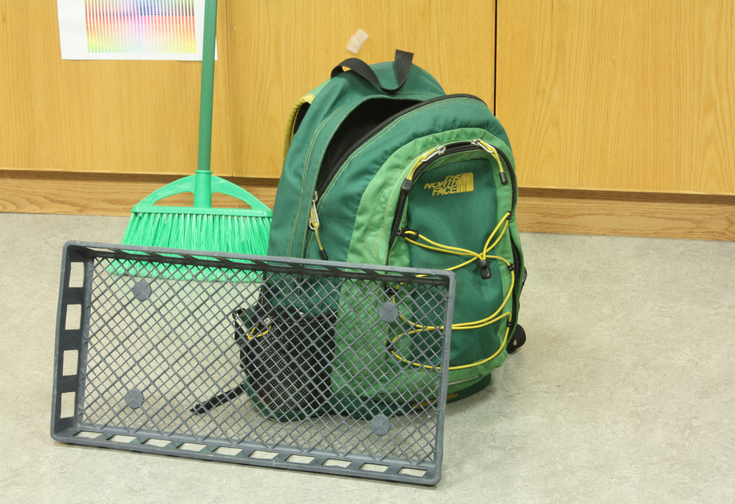
\includegraphics[scale=0.15]{./figures/im_left.png}
 		\caption{left image}
	\end{subfigure}
	\begin{subfigure}{0.49\linewidth}
		\centering
		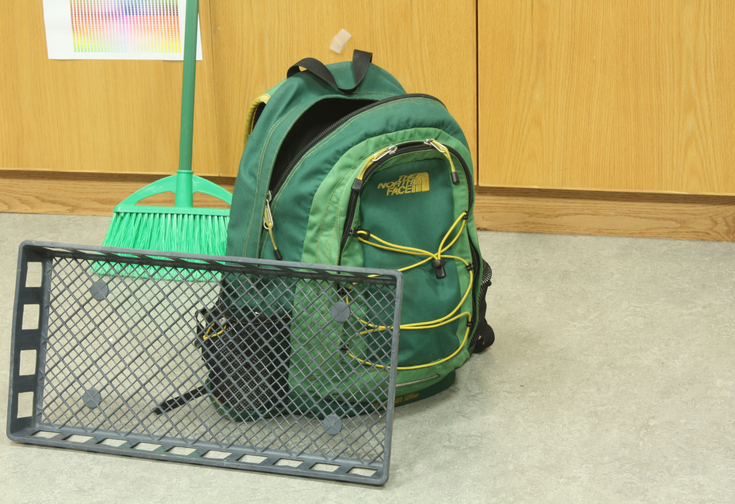
\includegraphics[scale=0.15]{./figures/im_right.png}
 		\caption{right image}
	\end{subfigure}
\caption{Given images for disparity map calculation}\label{fig:givenImages}
\end{figure}

\section{One thread implementation of ZNCC algorithm}\label{sec:CbasedImplementation}
\subsection{Area-based correspondence search}
The goal of the correspondence search is to find the corresponding pixel in the right image (a match) for the given pixel on the left image. Usually, comparing just pixels is not enough, therefore, their neighborhoods are compared.

In the area based matching algorithms, rectangular blocks of pixels from a set of two images $W \times H$ (left and right images) are compared and matched. We conducted our experiments for the images presented in Fig.~\ref{fig:givenImages}. For each block of the left image, designated by reference window, a corresponding block in the right image is sought. During the search process, the correspondent block of the right image is moved with a shift parameter $d$ and compared with the left block using some similarity measure $\otimes$. . In this work we will consider only rectified images, therefore there is no disparity and shift on the vertical axis.

 Let $\mathbf{L}_{xy}$ and $ \mathbf{R}_{xy}$ be blocks of the left and the right images respectively, centered at some point $(x, y)$ and $C_{xy}(d)$ -- a cost function of matching these blocks, defined by a similarity measure $\otimes$. The disparity field $\mathbf{D}$ is estimated then as

\begin{equation}
\mathbf{D} = \{ d_{xy}(d): 0\leq x < W; 0\leq y < H \},
\end{equation}
\noindent where 
\begin{equation}
d_{xy}(d) = \argmax{d}C_{xy}(d),
\end{equation}
\begin{equation}
C_{xy}(d) = \mathbf{L}_{xy}\otimes \mathbf{R}_{(x-d)y}.
\end{equation}

Many different similarity measures $\otimes$ have been referred in the literature~\cite{Redert99}. The reasons for a particular selection are usually related to the computational load, achieved performance and algorithmic simplicity. In this work we use ZNCC similarity measure:
\begin{equation}\label{eq:zncc}
ZNCC_{xy}(d)=\frac{\left(\mathbf{L}_{xy}-\overline{\mathbf{L}_{xy}}\right) * \left(\mathbf{R}_{(x-d)y}-\overline{\mathbf{R}_{(x-d)y}}\right)}
{\|\mathbf{L}_{xy}-\overline{\mathbf{L}_{xy}}\|_2 \|\mathbf{R}_{(x-d)y}-\overline{\mathbf{R}_{(x-d)y}}\|_2}
\end{equation}

\noindent where $\overline{\mathbf{L}_{xy}},\overline{\mathbf{R}_{xy}}$ -- block means.

Usually, the selection of the size of the reference window is not a simple and trivial task. It has been shown that the probability of a mismatch usually decreases as the size of the reference window increases. However, using large windows leads to an accuracy loss, since the influence of image differences increases greatly with the increase of the considered area. Therefore, this parameter must be great enough so that search window comprises the correspondent block of the given image. Furthermore, a difficult and important trade-off must be done when selecting this window size, since the computational load and processing time usually increase quadratically with the size of the window. Often, a compromise must be made, by adjusting these parameters according to the image size and contents. Taking into account all these factors and evaluating many experiments, we discovered that $15 \times 21$ is an optimal size of the window for our implementation and input data.

\subsection{ZNCC algorithm design}

\begin{figure}[t!]
\centering
	\begin{subfigure}{0.49\linewidth}
		\centering
		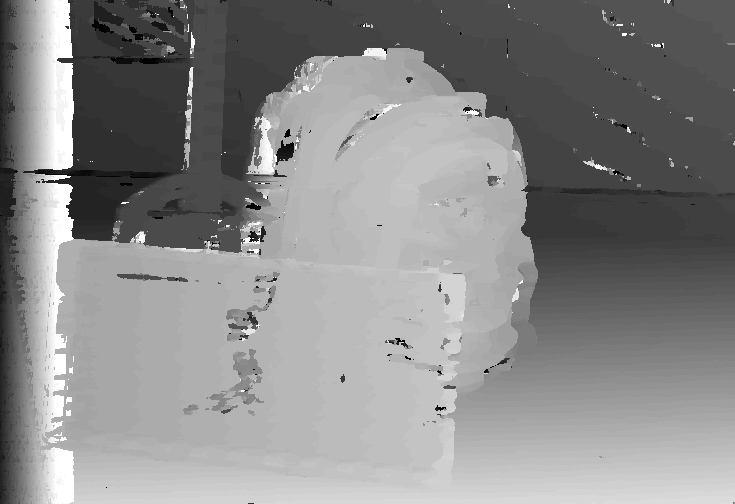
\includegraphics[scale=0.2]{./figures/left_dm.jpg}
 		\caption{Left disparity map}\label{subfig:leftDisparity}
	\end{subfigure}
	\begin{subfigure}{0.49\linewidth}
		\centering
		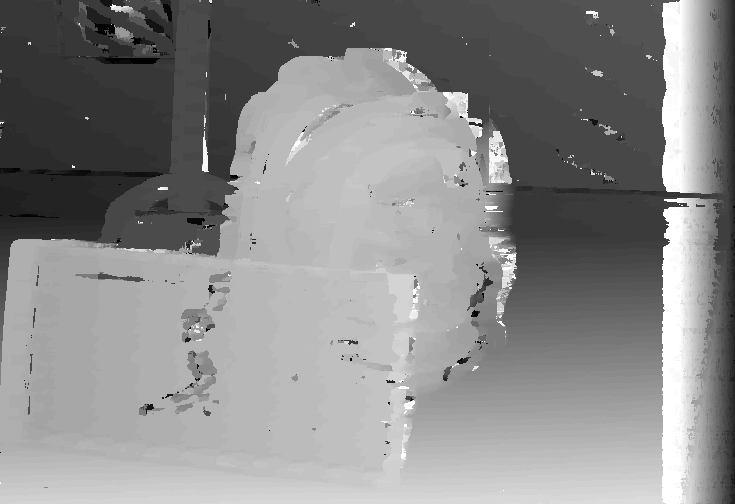
\includegraphics[scale=0.2]{./figures/right_dm.jpg}
 		\caption{Right disparity map}\label{subfig:rightDisparity}
	\end{subfigure}
\\
	\begin{subfigure}{\linewidth}
		\centering
		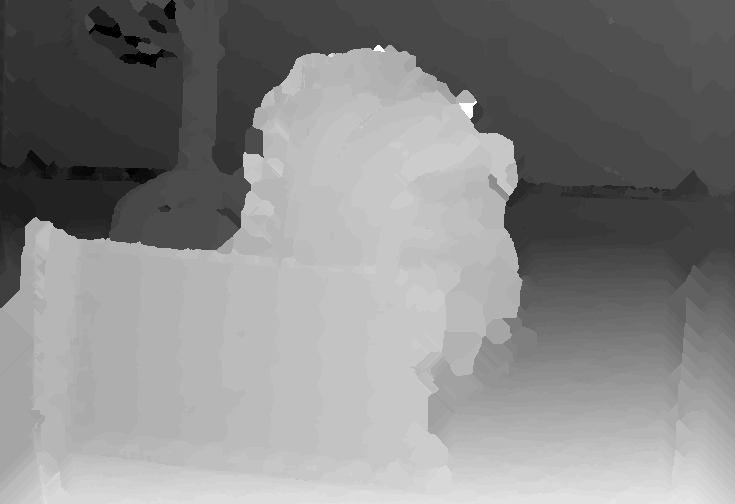
\includegraphics[scale=0.43]{./figures/final_dm.jpg}
 		\caption{The final disparity map}\label{subfig:finalDisparity}
	\end{subfigure}
\caption{Given images for disparity map calculation}\label{fig:disparities}
\end{figure}

The original images were scaled to a smaller size (4 times) in order to decrease computational time. Next, utilizing Eq.~\ref{eq:zncc}, we calculated disparity maps for both of the images and for a disparity value \textit{d} from 0 to 64. The results are illustrated in Fig.~\ref{subfig:leftDisparity} and Fig.~\ref{subfig:rightDisparity} respectively. In order to compute Right-Left disparity we made a trick with setting up a disparity range. Specifically, the lower bound was initialized to -64 and the upper bound to 0. Once disparity maps for both images were computed, we perform post-processing consisting of two stages: cross-checking and occlusion filling. Cross-checking is calculated by taking the computed disparity value in one image, and re-projecting it in the other image. If the difference in the values is higher than a given threshold (equals to 2 in our work), then the pixel value is initialized to 0. Occlusion filling was performed by applying the nearest neighbor interpolation. Neighborhood was chosen to be a square block $256\times256$. The final disparity map is illustrated in Fig.~\ref{subfig:finalDisparity}. 

Visually, we can observe, that our result looks quite good after post-processing steps, however, the computational load and elapsed time for this implementation are remarkably high -- more than one minute. In the following section, we propose an approach for acceleration of our implementation of ZNCC algorithm based on OpenCL technology which significantly improves performance.

\section{OpenCL implementation}\label{sec:OpenclImplementation}
\subsection{Description}
In terms of OpenCL, there are two types of devices -- host and device. In our case, the device was a GPU and host -- Central Processor (CPU).

We have decided to create a separate kernel for each of the sub-problems of our implementation (resizing, zncc computation, cross-checking and occlusion filling): \textit{resize.cl}, \textit{zncc.cl}, \textit{cross\_check.cl} and \textit{occlusion.cl} respectively. We performed normalization of the disparity map (between 0 and 255) on the host, since it would take a lot of efforts to implement it in OpenCL and it would not give a significant performance improvement. The structure of the host code is presented in Algorithm \ref{hostcode}.


 \begin{algorithm}
 \caption{Host algorithm}\label{hostcode}
 \begin{algorithmic}[1]
 \renewcommand{\algorithmicrequire}{\textbf{Input:}}
 \renewcommand{\algorithmicensure}{\textbf{Output:}}
 \REQUIRE Images filenames.
  \STATE Check arguments.
  \STATE Read images.
  \STATE Chose the vendor and the device.
  \STATE Allocate memory on the device for the original images and the intermediate results.
  \STATE Copy the original images to the device, to the certain preallocated buffers.
  \STATE Consequently set arguments load kernels to the queue.
  \STATE Wait until the kernels execution is finished.
  \STATE Copy the result into host memory.
  \STATE Normalize the disparity map.
  \STATE Save the result to \textit{depthmap.png}.
 \end{algorithmic} 
 \end{algorithm}

\section{Optimization of OpenCL kernels}\label{sec:Optimization}
\subsection{Local memory tricks} 
In our work we did not use any local memory tricks, but the potential usage of it would be in caching the blocks for the calculation of mean and standard deviation.

\subsection{If-statements removal}
First kernel optimization which we have made was removing extra if-statements  which check the image boundaries. The outcome of such modification was a slight performance improvement (5\%, improved value is presented in Table \ref{benchnaive}).

\subsection{Work-group optimization}
We considered work-groups sizes to be divisors of width and height of the resized images. As a global size we took the new image size -- $504\times735$. We enumerated all possible values of work-group sizes using divisors of 504 and 735 and found, that the work group size giving the best performance in our implementation of ZNCC is $3\times21$. The number of work-items in such a work-group is almost equal to 64, which is recommended by NVIDIA.


\section{Benchmarks}\label{sec:Benchmarks}
We have tested our OpenCL implementation on two different machines with Ubuntu 14.04 64 bit. Both machines have NVIDIA GPUs, the same version graphics drivers and CUDA 7.5. We also ran our implementation on the laptop with Intel CPU 6200U Skylake. However, OpenCL implementation turned out to be slower than the original C version. Presumably, it happened due to the communication overhead. We could have improved the benchmark result, but decided to focus only on GPU implementations. Our benchmark results (average of 3 launches) are presented in Table \ref{benchnaive}.
\begin{table}
\caption{Benchmarking of the naive OpenCL implementation}\label{benchnaive}
\centering
\begin{tabular}
{|c|C{1.5cm}|C{1.5cm}|C{1cm}|}
\hline
{\bfseries Device}  & {\bfseries Plain C time [sec]}  & {\bfseries GPU time [sec]} & {\bfseries Performance gain} \\
\hline
NVIDIA GTX960 OC & 84.9350 & 0.8356 & 101.65\\
\hline
NVIDIA GTX750 Titan & 77.5322 & 1.7745 & 43.7\\
\hline
\end{tabular}
\end{table}

In our testing equipment, the machine with the more powerful GPU had less powerful CPU than the machine with GTX750 (Intel(R) Core(TM) i5-3470 vs. Intel(R) Core(TM) i5-4570). By changing the processors, our performance gain would be still good -- 92.79. In our work we report it as a final result.


\section{Compiling and running}

We have tested our implementation on the following software: Ubuntu 14.04 64 bit, GCC compiler version 4.8.4, NVIDIA drivers 352.93, NVIDIA CUDA 7.5. In order to compile the code, the user just need to use \textit{make} utility (see the Listing \ref{mylisting}).

\begin{lstlisting}[language=bash,caption={Compiling commands},label={mylisting}]
# Compile and run OpenCL code
make cl runcl
# Compile and run plain C code
make c runc
\end{lstlisting}

Our implementations of ZNCC are available on GitHub. The code is available by the following link -- \url{https://github.com/lext/zncc}

\section{Discussion and Conclusions}
In this work we have presented an implementation of ZNCC algorithm using OpenCL. Despite the fact that we did not use any local memory tricks, which usually give a good performance gain, we have shown, that it is possible to  achieve a quite good result even without them -- 92.79 on a machine with Intel(R) Core(TM) i5-4570 CPU @ 3.20GHz and GPU NVIDIA GTX960. We have also shown, that by changing the GPU to the newer generation, our performance gain has increased more than twice.

\bibliographystyle{IEEEtran}
\bibliography{report}

\end{document}


